%%
% Master's Thesis Defense Presentation
% Using TUM Corporate Design LaTeX Template (tumbeamer)
%%

\documentclass[
  english,
  aspectratio=169,
]{tumbeamer}

% load additional packages
\usepackage{booktabs}
\usepackage{amsmath}
\usepackage{multirow}
\usepackage{graphicx}
\usepackage{xcolor}
\usepackage{tcolorbox}


% presentation metadata
\title{Learning Camera Geometry from Unlabeled Real-World Dynamic Video}
\subtitle{Master's Thesis Defense}
\author{Kalman Eddi Mahlich}

\institute{%
  Supervisor: Prof.\ Dr.\ Daniel Cremers \quad Advisor: Daniil Sinitsyn\\[2pt]
  \theChairName\\
  \theDepartmentName\\
  \theUniversityName%
}
\date[14/03/2026]{March 14, 2026}

\footline{\insertauthor~|~\insertshorttitle~|~\insertshortdate}


% macro to configure the style of the presentation
\TUMbeamersetup{
  title page = TUM tower,
  part page = TUM toc,
  section page = TUM toc,
  content page = TUM more space,
  tower scale = 1.0,
  headline = TUM threeliner,
  footline = TUM default,
  headline on = {title page},
  footline on = {every page, title page=false},
}


\begin{document}

% ============================================================================
% SLIDE 1: Title
% ============================================================================
\maketitle


% ============================================================================
% SLIDE 2: Outline
% ============================================================================
\begin{frame}{Outline}

\begin{enumerate}
  \setlength{\itemsep}{8pt}
  \item Motivation \& Background
  \item AnyCam Baseline
  \item Our Idea: Integrating AnyCalib
  \item Method Overview \& Contributions
  \item Training Setup
  \item Results
  \item Conclusion \& Future Work
\end{enumerate}

\end{frame}


% ============================================================================
% SLIDE 3: Motivation — Introduction
% ============================================================================
\begin{frame}{Motivation}

Recovering \textbf{camera geometry} from video is fundamental to 3D vision.

\vskip4pt
% TODO: Replace placeholder with a visual collage/strip showing
% application domains: autonomous driving, AR, robotics, 3D reconstruction
% (e.g., 4 example images side by side)
\begin{center}
\fcolorbox{TUMBlue}{TUMBlue!5}{%
\begin{minipage}{0.88\textwidth}
\centering\vskip6pt
{\small\color{TUMBlue}\textbf{[ Visual: application domains --- driving, AR, robotics, 3D reconstruction ]}}
\vskip6pt
\end{minipage}%
}
\end{center}

\vskip4pt
\begin{columns}[T]
\begin{column}{0.55\textwidth}
\textbf{The challenge:} casual video means
\begin{itemize}
  \item Unknown camera parameters
  \item Dynamic scenes
  \item No labels at scale
\end{itemize}
\end{column}

\begin{column}{0.43\textwidth}
\textbf{AnyCam} [CVPR 2025] is the SOTA\\self-supervised method for this.

\vskip4pt
But its calibration is a bottleneck ---\\let me show you why.
\end{column}
\end{columns}

\end{frame}


% ============================================================================
% SLIDE 4: The Calibration Problem
% ============================================================================
\begin{frame}{The Calibration Problem in AnyCam}

\begin{center}
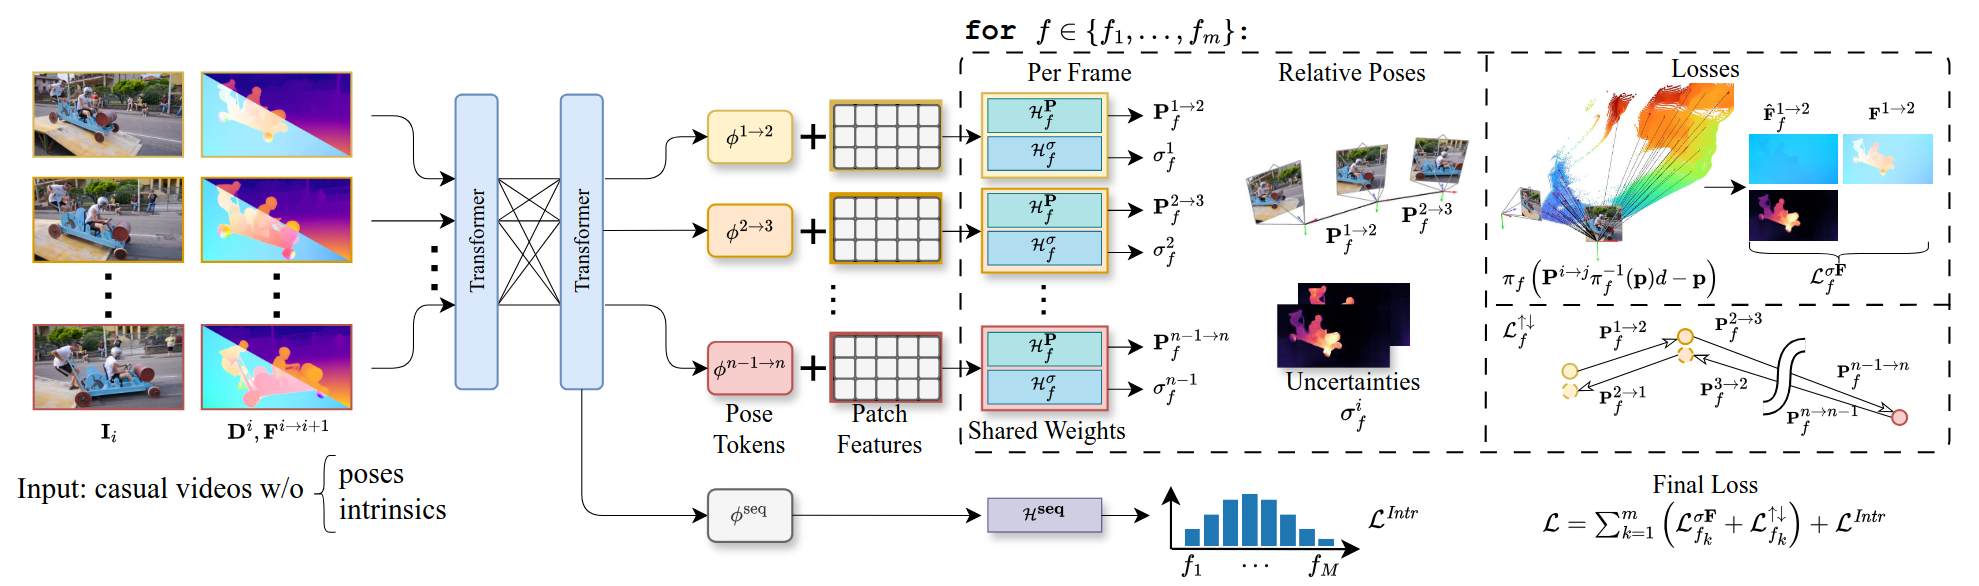
\includegraphics[width=0.68\textwidth]{figures/anycam_pipeline.png}
{\tiny \quad [Wimbauer et al., CVPR 2025]}
\end{center}

\vskip-4pt
\begin{columns}[T]
\begin{column}{0.52\textwidth}
\textbf{AnyCam's 32-candidate system:}
\begin{itemize}
  \item Generates 32 focal length guesses
  \item Runs flow reprojection for each
  \item Picks the one with lowest error
\end{itemize}
Expensive, coarse, and often wrong.
\end{column}

\begin{column}{0.44\textwidth}
\textbf{How wrong?}
\vskip1pt
\centering
\footnotesize
\begin{tabular}{lc}
  \toprule
  Dataset & AnyCam MAPE \\
  \midrule
  Sintel & \alert{45.1\%} \\
  TUM-RGBD & \alert{63.7\%} \\
  \bottomrule
\end{tabular}
\vskip2pt
\flushleft
Better calibration $\to$ \textbf{better poses}.
\end{column}
\end{columns}

\end{frame}


% ============================================================================
% SLIDE 5: AnyCalib — Fixing the Calibration
% ============================================================================
\begin{frame}{AnyCalib --- A Path to Better Calibration}

\textbf{AnyCalib} [Tirado-Gar\'in \& Civera, 2025] --- model-agnostic single-image calibration:

\vskip2pt
\begin{center}
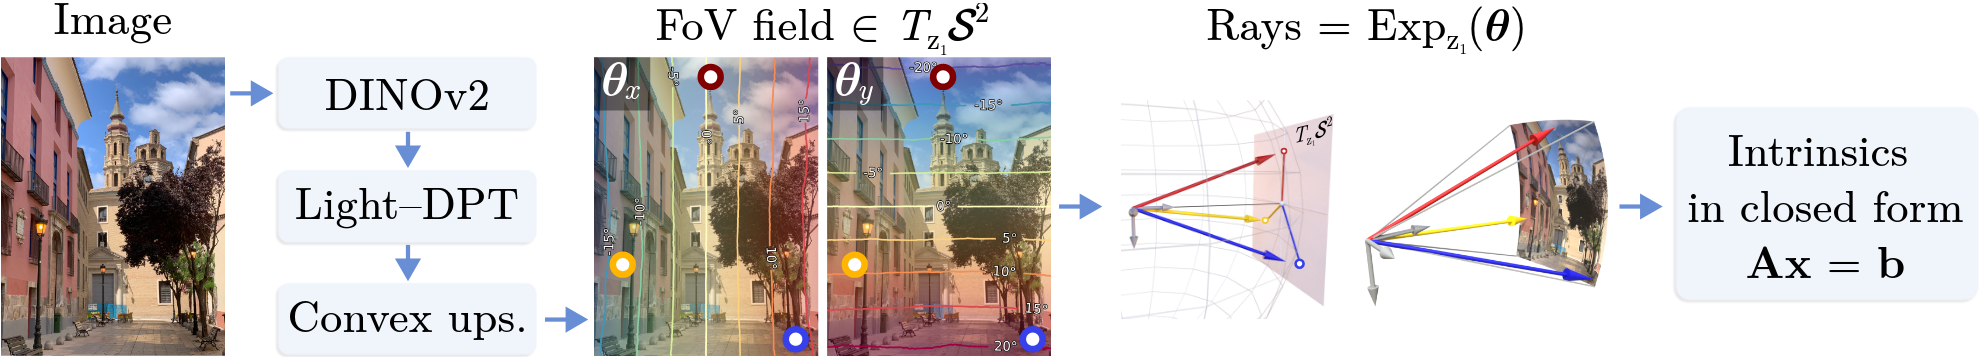
\includegraphics[width=0.78\textwidth]{figures/anycalib_pipeline.png}
\vskip1pt
{\tiny Single image $\to$ DINOv2 ViT-L $\to$ DPT $\to$ per-pixel rays $\to$ closed-form $\mathbf{K}$}
\end{center}

\vskip4pt
\begin{columns}[T]
\begin{column}{0.48\textwidth}
Much better calibration than AnyCam.\\[2pt]
Even naive per-frame averaging helps.
\end{column}

\begin{column}{0.48\textwidth}
\textbf{But:} per-frame only --- noisy, no consistency.\\[2pt]
What if we leverage \textbf{multi-frame consistency}?\\[2pt]
$\to$ Our method: \textbf{MCT} on AnyCalib's features.
\end{column}
\end{columns}

\end{frame}


% ============================================================================
% SLIDE 6: Our Method --- Pipeline
% ============================================================================
\begin{frame}{Our Method --- Complete Pipeline}

% TODO: Replace with actual pipeline diagram showing:
%   Two parallel branches from N input frames:
%   - Pose:  DINOv2-small (frozen) -> Pose Neck (train) -> Pose Head (train) -> R, t
%   - Calib: DINOv2 ViT-L (frozen) -> [MCT] (train) -> DPT (frozen) -> rays -> K
%   Plus: UniDepth (frozen) for depth, UniMatch (frozen) for optical flow
%   Flow reprojection loss connects both branches (self-supervised)
%   Show frozen components grayed out, trainable in color

\begin{center}
\fcolorbox{TUMBlue}{TUMBlue!5}{%
\begin{minipage}{0.88\textwidth}
\centering\vskip8pt
{\large\color{TUMBlue}\textbf{[ Pipeline diagram to be inserted ]}}
\vskip12pt
\small
\textbf{Pose branch:} DINOv2-small $\to$ Pose Neck $\to$ Pose Head $\to$ $\mathbf{R}, \mathbf{t}$\\[3pt]
\textbf{Calibration branch:} DINOv2 ViT-L $\to$ \textbf{MCT} $\to$ DPT decoder $\to$ $\mathbf{K}$\\[3pt]
Self-supervised via flow reprojection loss
\vskip8pt
\end{minipage}%
}
\end{center}

\end{frame}


% ============================================================================
% SLIDE 7: Contributions
% ============================================================================
\begin{frame}{Contributions}

\begin{columns}[T]
\begin{column}{0.48\textwidth}

\textbf{1. AnyCalib $\boldsymbol{\times}$ AnyCam}
\begin{itemize}
  \item Inject AnyCalib's accurate calibration directly into AnyCam's projection matrix
  \item Improves both pose and calibration
\end{itemize}

\vskip8pt
\textbf{2. Multi-Frame Calibration Transformer}
\begin{itemize}
  \item Cross-frame attention on AnyCalib's backbone features (4 scales)
  \item Enforces calibration consistency across frames
  \item Improves further on per-frame AnyCalib
\end{itemize}

\end{column}

\begin{column}{0.50\textwidth}
\centering
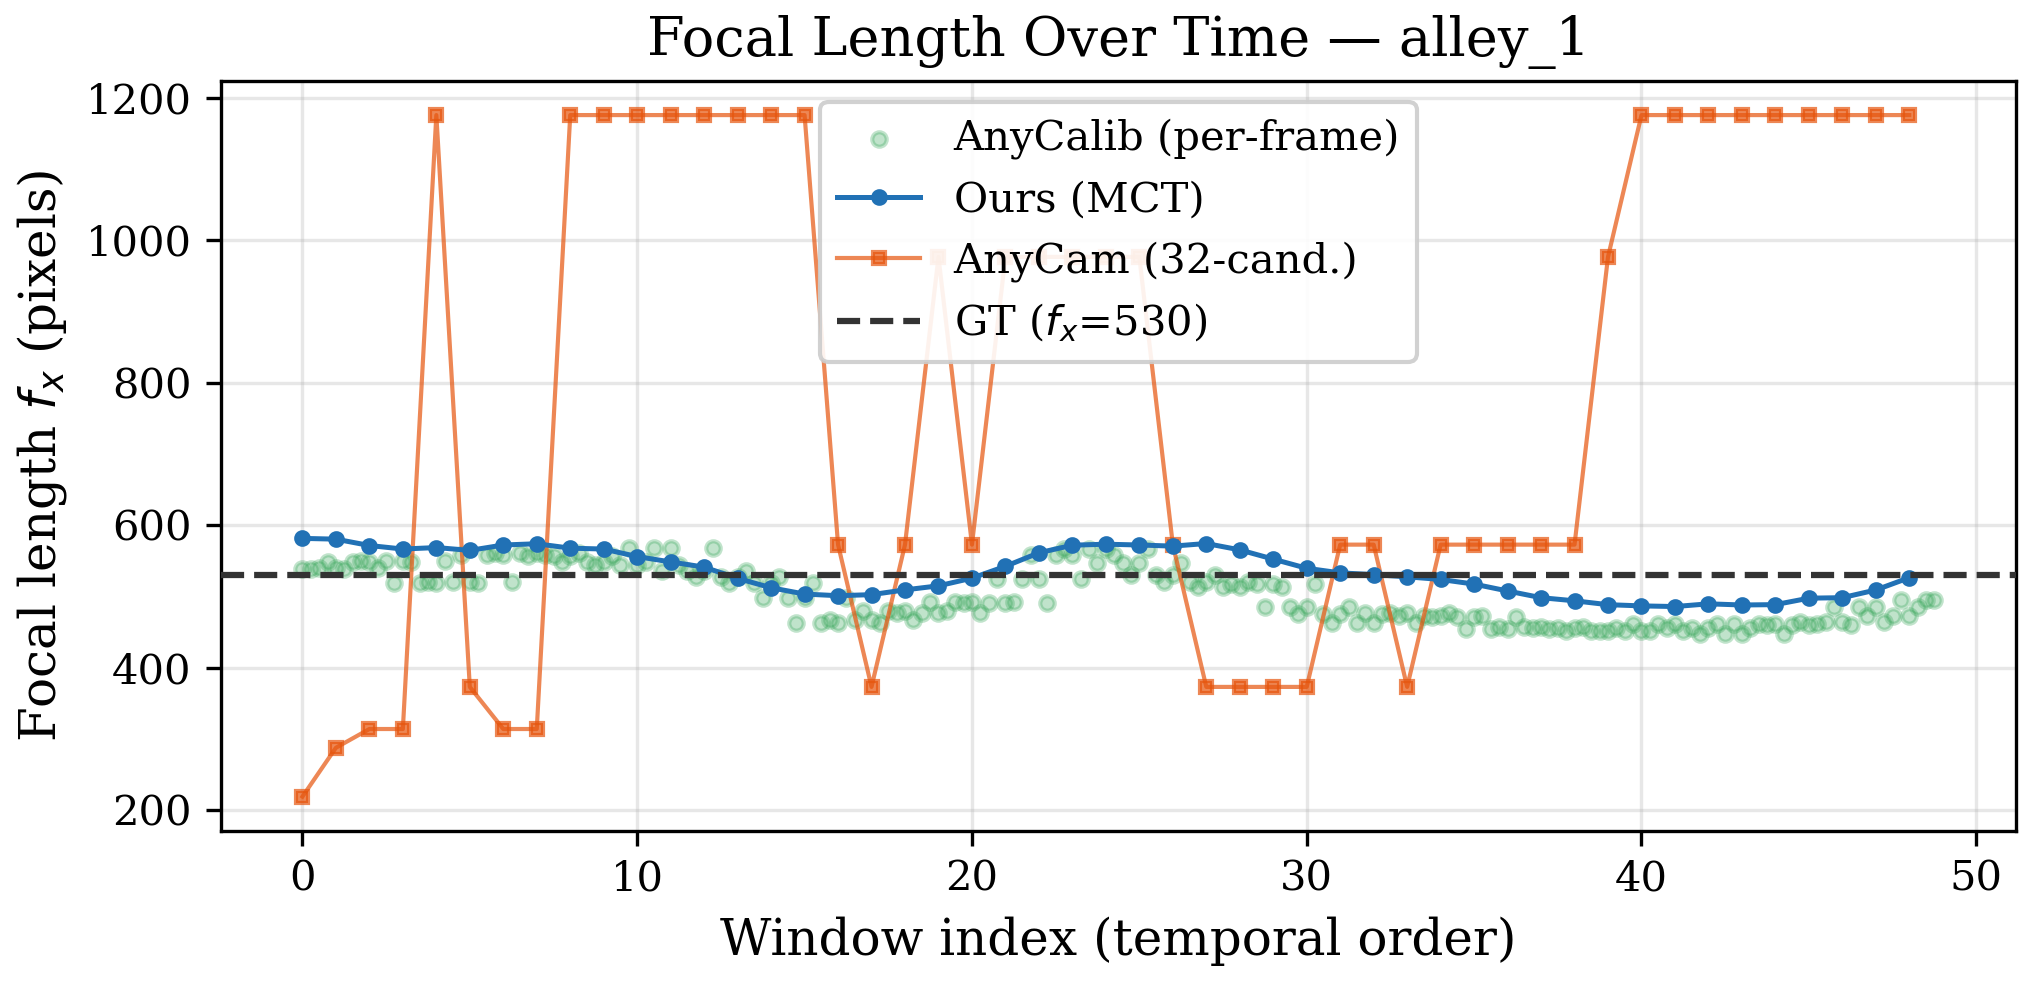
\includegraphics[width=\textwidth]{figures/focal_length_over_time.png}
\vskip4pt
{\small MCT (blue): smooth, accurate.\\
AnyCalib per-frame (green): noisy.\\
AnyCam 32-cand.\ (orange): large outliers.}
\end{column}
\end{columns}

\end{frame}


% ============================================================================
% SLIDE 8: Training
% ============================================================================
\begin{frame}{Training Setup}

% TODO: Replace with a training/architecture diagram showing:
%   - Frozen components (grayed): DINOv2 backbones, DPT, UniDepth, UniMatch (~340M)
%   - Trainable components (colored): Pose Neck (~2.5M), Pose Head (~21K), MCT (~25M)
%   - Loss arrows: flow reprojection (self-supervised) + calibration anchor (AnyCalib pseudo-GT)
%   - Total: ~27.5M / 370M trainable (7.5%)

\begin{center}
\fcolorbox{TUMBlue}{TUMBlue!5}{%
\begin{minipage}{0.88\textwidth}
\centering\vskip8pt
{\large\color{TUMBlue}\textbf{[ Training diagram to be inserted ]}}
\vskip12pt
\small
Frozen (gray): DINOv2 backbones, DPT, UniDepth, UniMatch (${\sim}340$M)\\[3pt]
Trained (color): Pose Neck, Pose Head, MCT (${\sim}27.5$M --- \textbf{7.5\%} of total)\\[3pt]
Loss: flow reprojection (self-supervised) + calibration anchor
\vskip8pt
\end{minipage}%
}
\end{center}

\vskip4pt
\begin{columns}[T]
\begin{column}{0.48\textwidth}
\begin{itemize}
  \item Self-supervised, like AnyCam
  \item Additional calibration anchor loss (AnyCalib pseudo-GT)
  \item 4 datasets, 82K frames
\end{itemize}
\end{column}

\begin{column}{0.48\textwidth}
\begin{itemize}
  \item Only 7.5\% of parameters trained
  \item No weeks of training needed
  \item Both backbones stay frozen
\end{itemize}
\end{column}
\end{columns}

\end{frame}


% ============================================================================
% SLIDE 9: Results --- Pose
% ============================================================================
\begin{frame}{Results --- Pose Accuracy}

\begin{columns}[T]
\begin{column}{0.48\textwidth}
\centering
\footnotesize
\begin{tabular}{lcc}
  \toprule
  Dataset & Rot.\ Mean/Med ($^\circ$) & Improv. \\
  \midrule
  Sintel & 0.88/0.30 $\to$ \textbf{0.60/0.19} & \alert{31.7\%} \\
  TUM-RGBD & 2.03/1.23 $\to$ \textbf{1.39/0.71} & \alert{31.5\%} \\
  KITTI & 0.56/0.26 $\to$ \textbf{0.54/0.25} & 3.6\% \\
  \bottomrule
\end{tabular}
\vskip2pt
{\tiny Rotation error ($\downarrow$ better). $N=200$ sequences per dataset.}

\vskip4pt
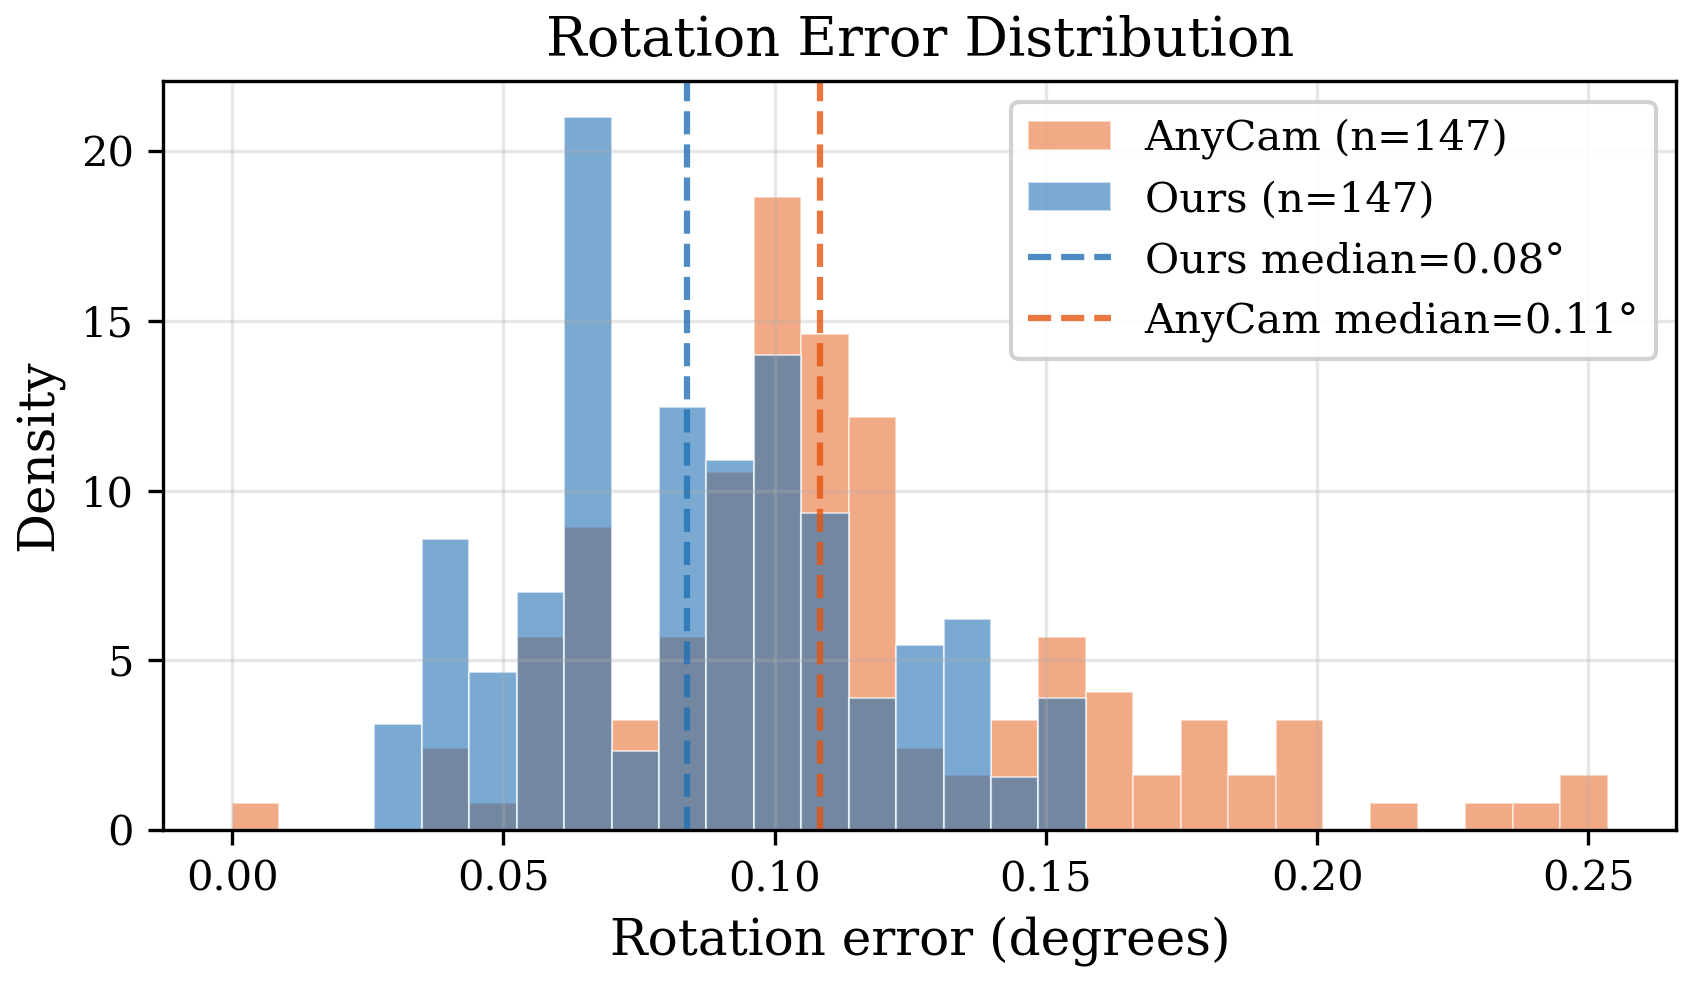
\includegraphics[width=\textwidth]{figures/rotation_error_histogram.png}
\end{column}

\begin{column}{0.48\textwidth}
\centering
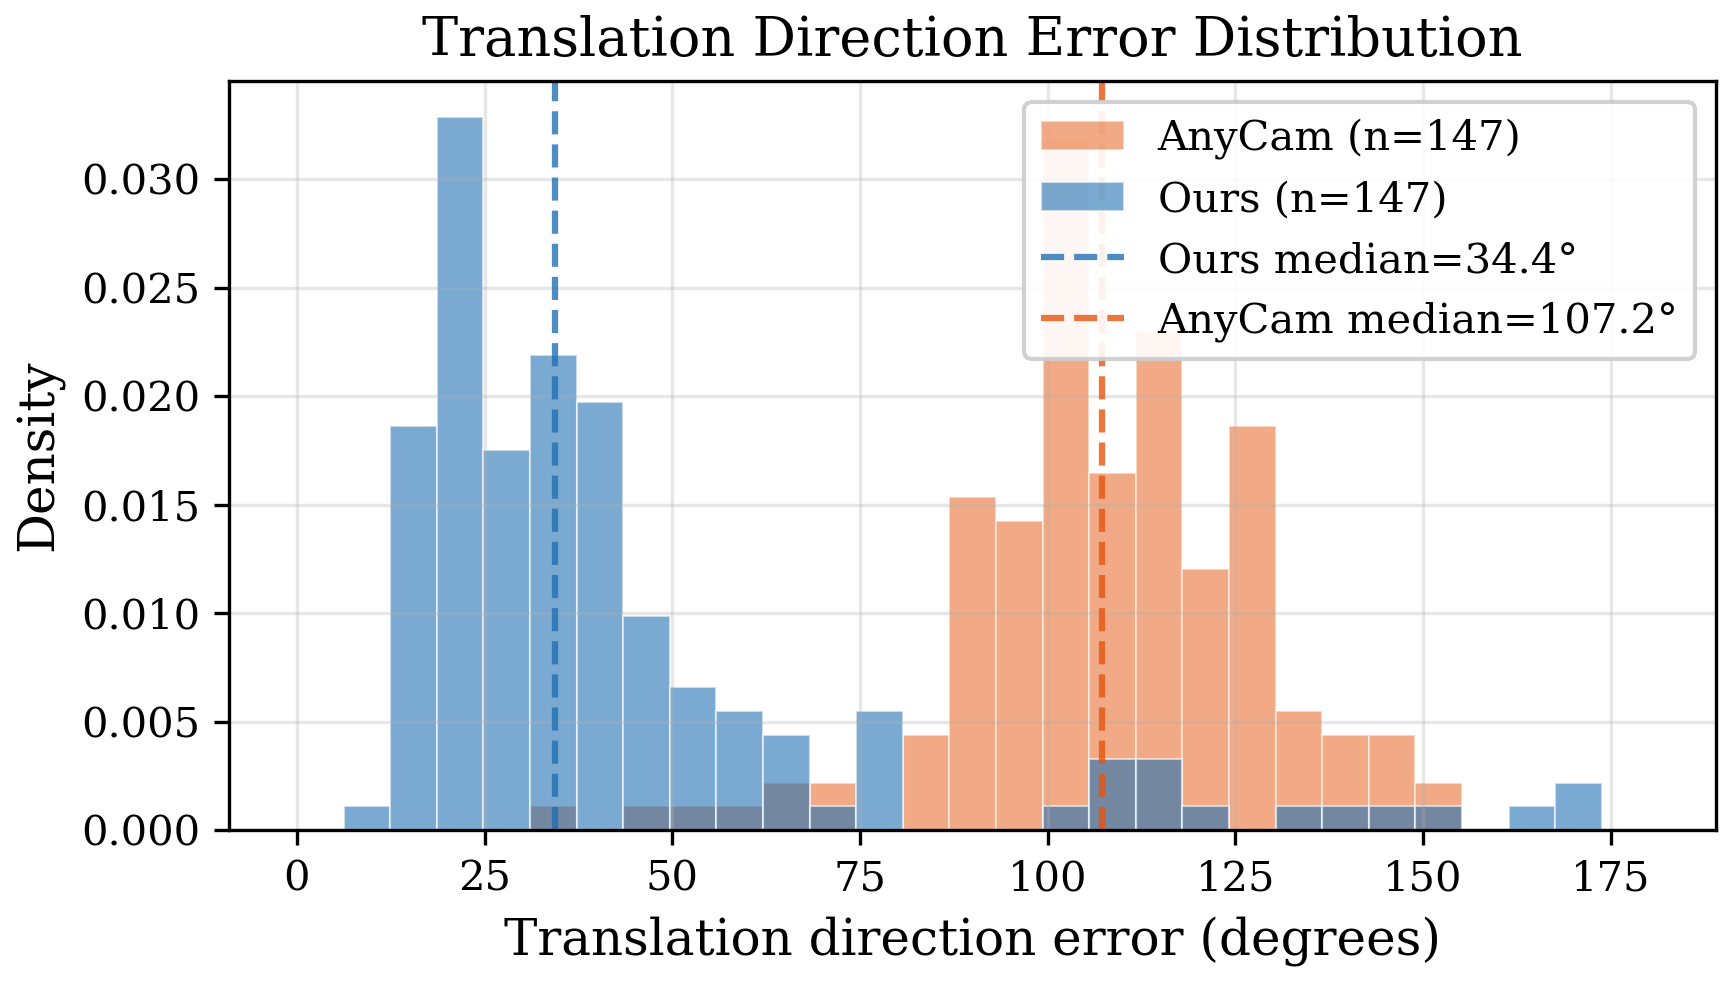
\includegraphics[width=\textwidth]{figures/translation_error_histogram.png}
\vskip4pt
\begin{itemize}\small
  \item Up to \textbf{31.7\% rotation error reduction}
  \item Consistent across all three datasets
  \item Largest gains on diverse scenes
\end{itemize}
\end{column}
\end{columns}

\end{frame}


% ============================================================================
% SLIDE 10: Results --- Calibration
% ============================================================================
\begin{frame}{Results --- Calibration Accuracy}

\begin{columns}[T]
\begin{column}{0.48\textwidth}
\centering
\small
\begin{tabular}{llcc}
  \toprule
  Dataset & Method & MAE & MAPE \\
  \midrule
  \multirow{3}{*}{Sintel}
  & AnyCam & 559.3 & 45.1\% \\
  & AnyCalib & 426.1 & 30.7\% \\
  & \textbf{Ours} & \textbf{300.3} & \textbf{27.8\%} \\
  \midrule
  \multirow{3}{*}{TUM}
  & AnyCam & 234.1 & 63.7\% \\
  & AnyCalib & 46.3 & 11.7\% \\
  & \textbf{Ours} & \textbf{30.3} & \textbf{7.9\%} \\
  \bottomrule
\end{tabular}
\vskip2pt
{\tiny $f_x$ MAE in pixels, combined $f$ MAPE (\%).}

\vskip4pt
Up to \textbf{32.5\% MAPE improvement} over AnyCalib.
\end{column}

\begin{column}{0.50\textwidth}
\centering
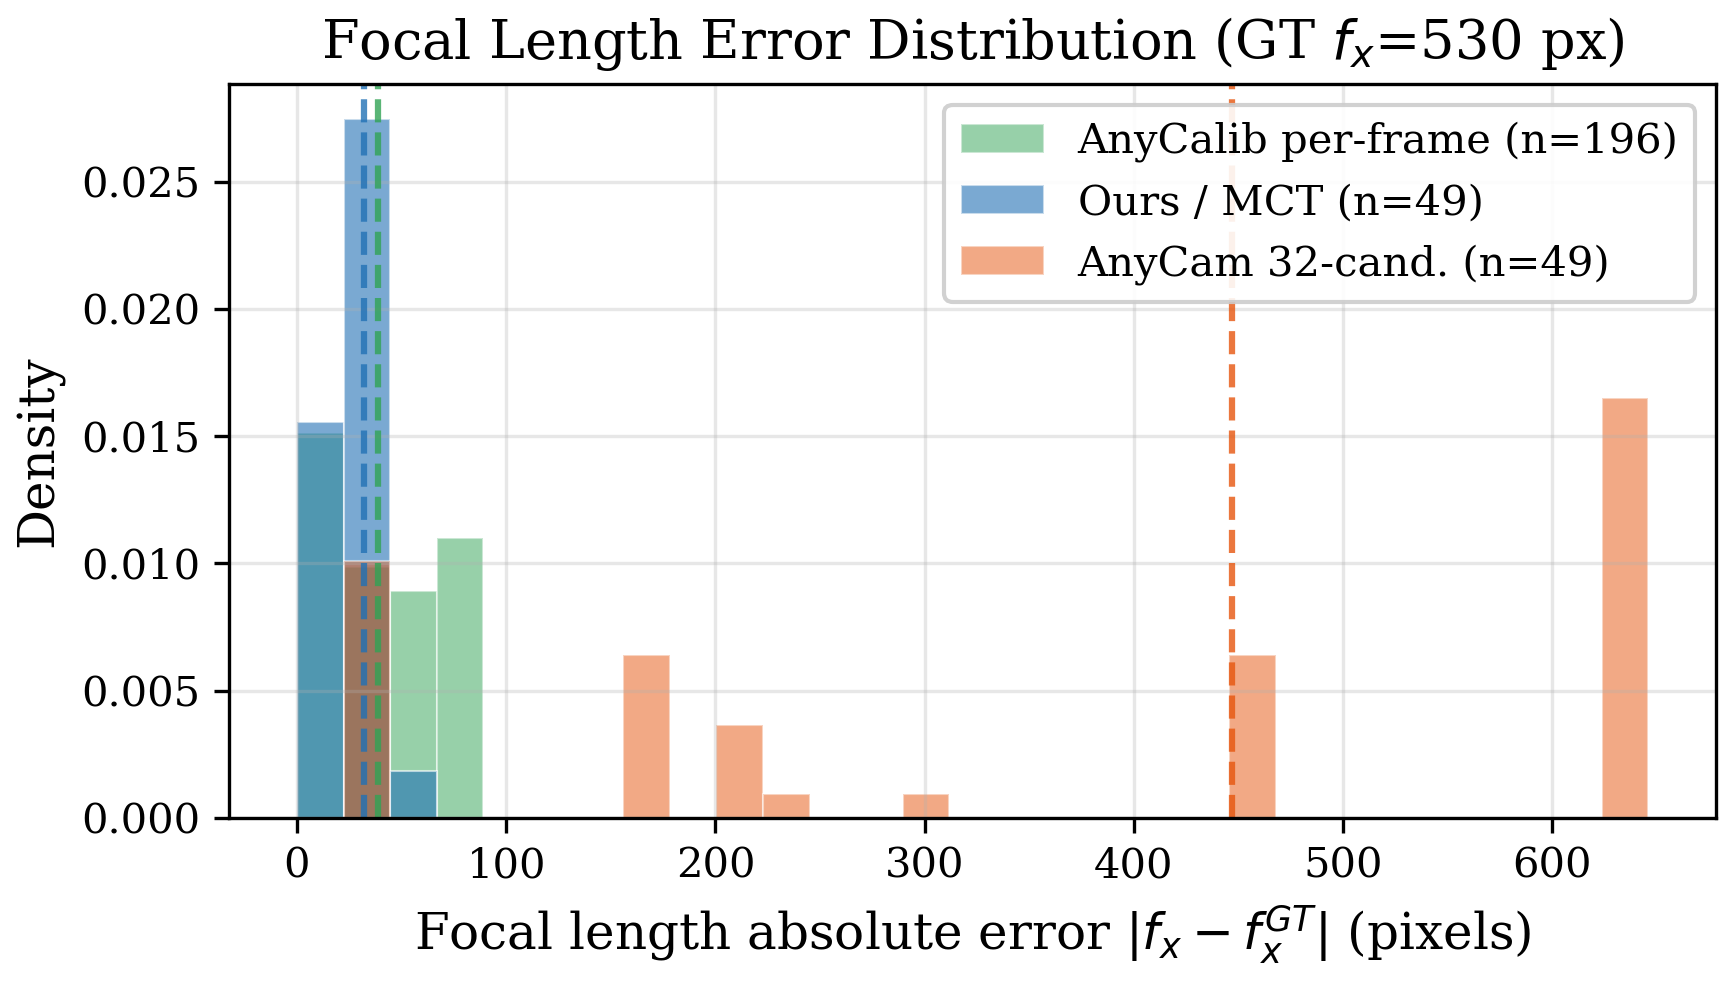
\includegraphics[width=\textwidth]{figures/focal_length_error_histogram.png}
\vskip2pt
{\small MCT errors near zero; AnyCam spread wide.}
\vskip4pt
\textbf{Key insight:} Feature-level aggregation preserves geometric structure lost in scalar averaging.
\end{column}
\end{columns}

\end{frame}


% ============================================================================
% SLIDE 11: Trajectory Visualization
% ============================================================================
\begin{frame}{Trajectory Visualization}

\begin{columns}[c]
\begin{column}{0.55\textwidth}
\centering
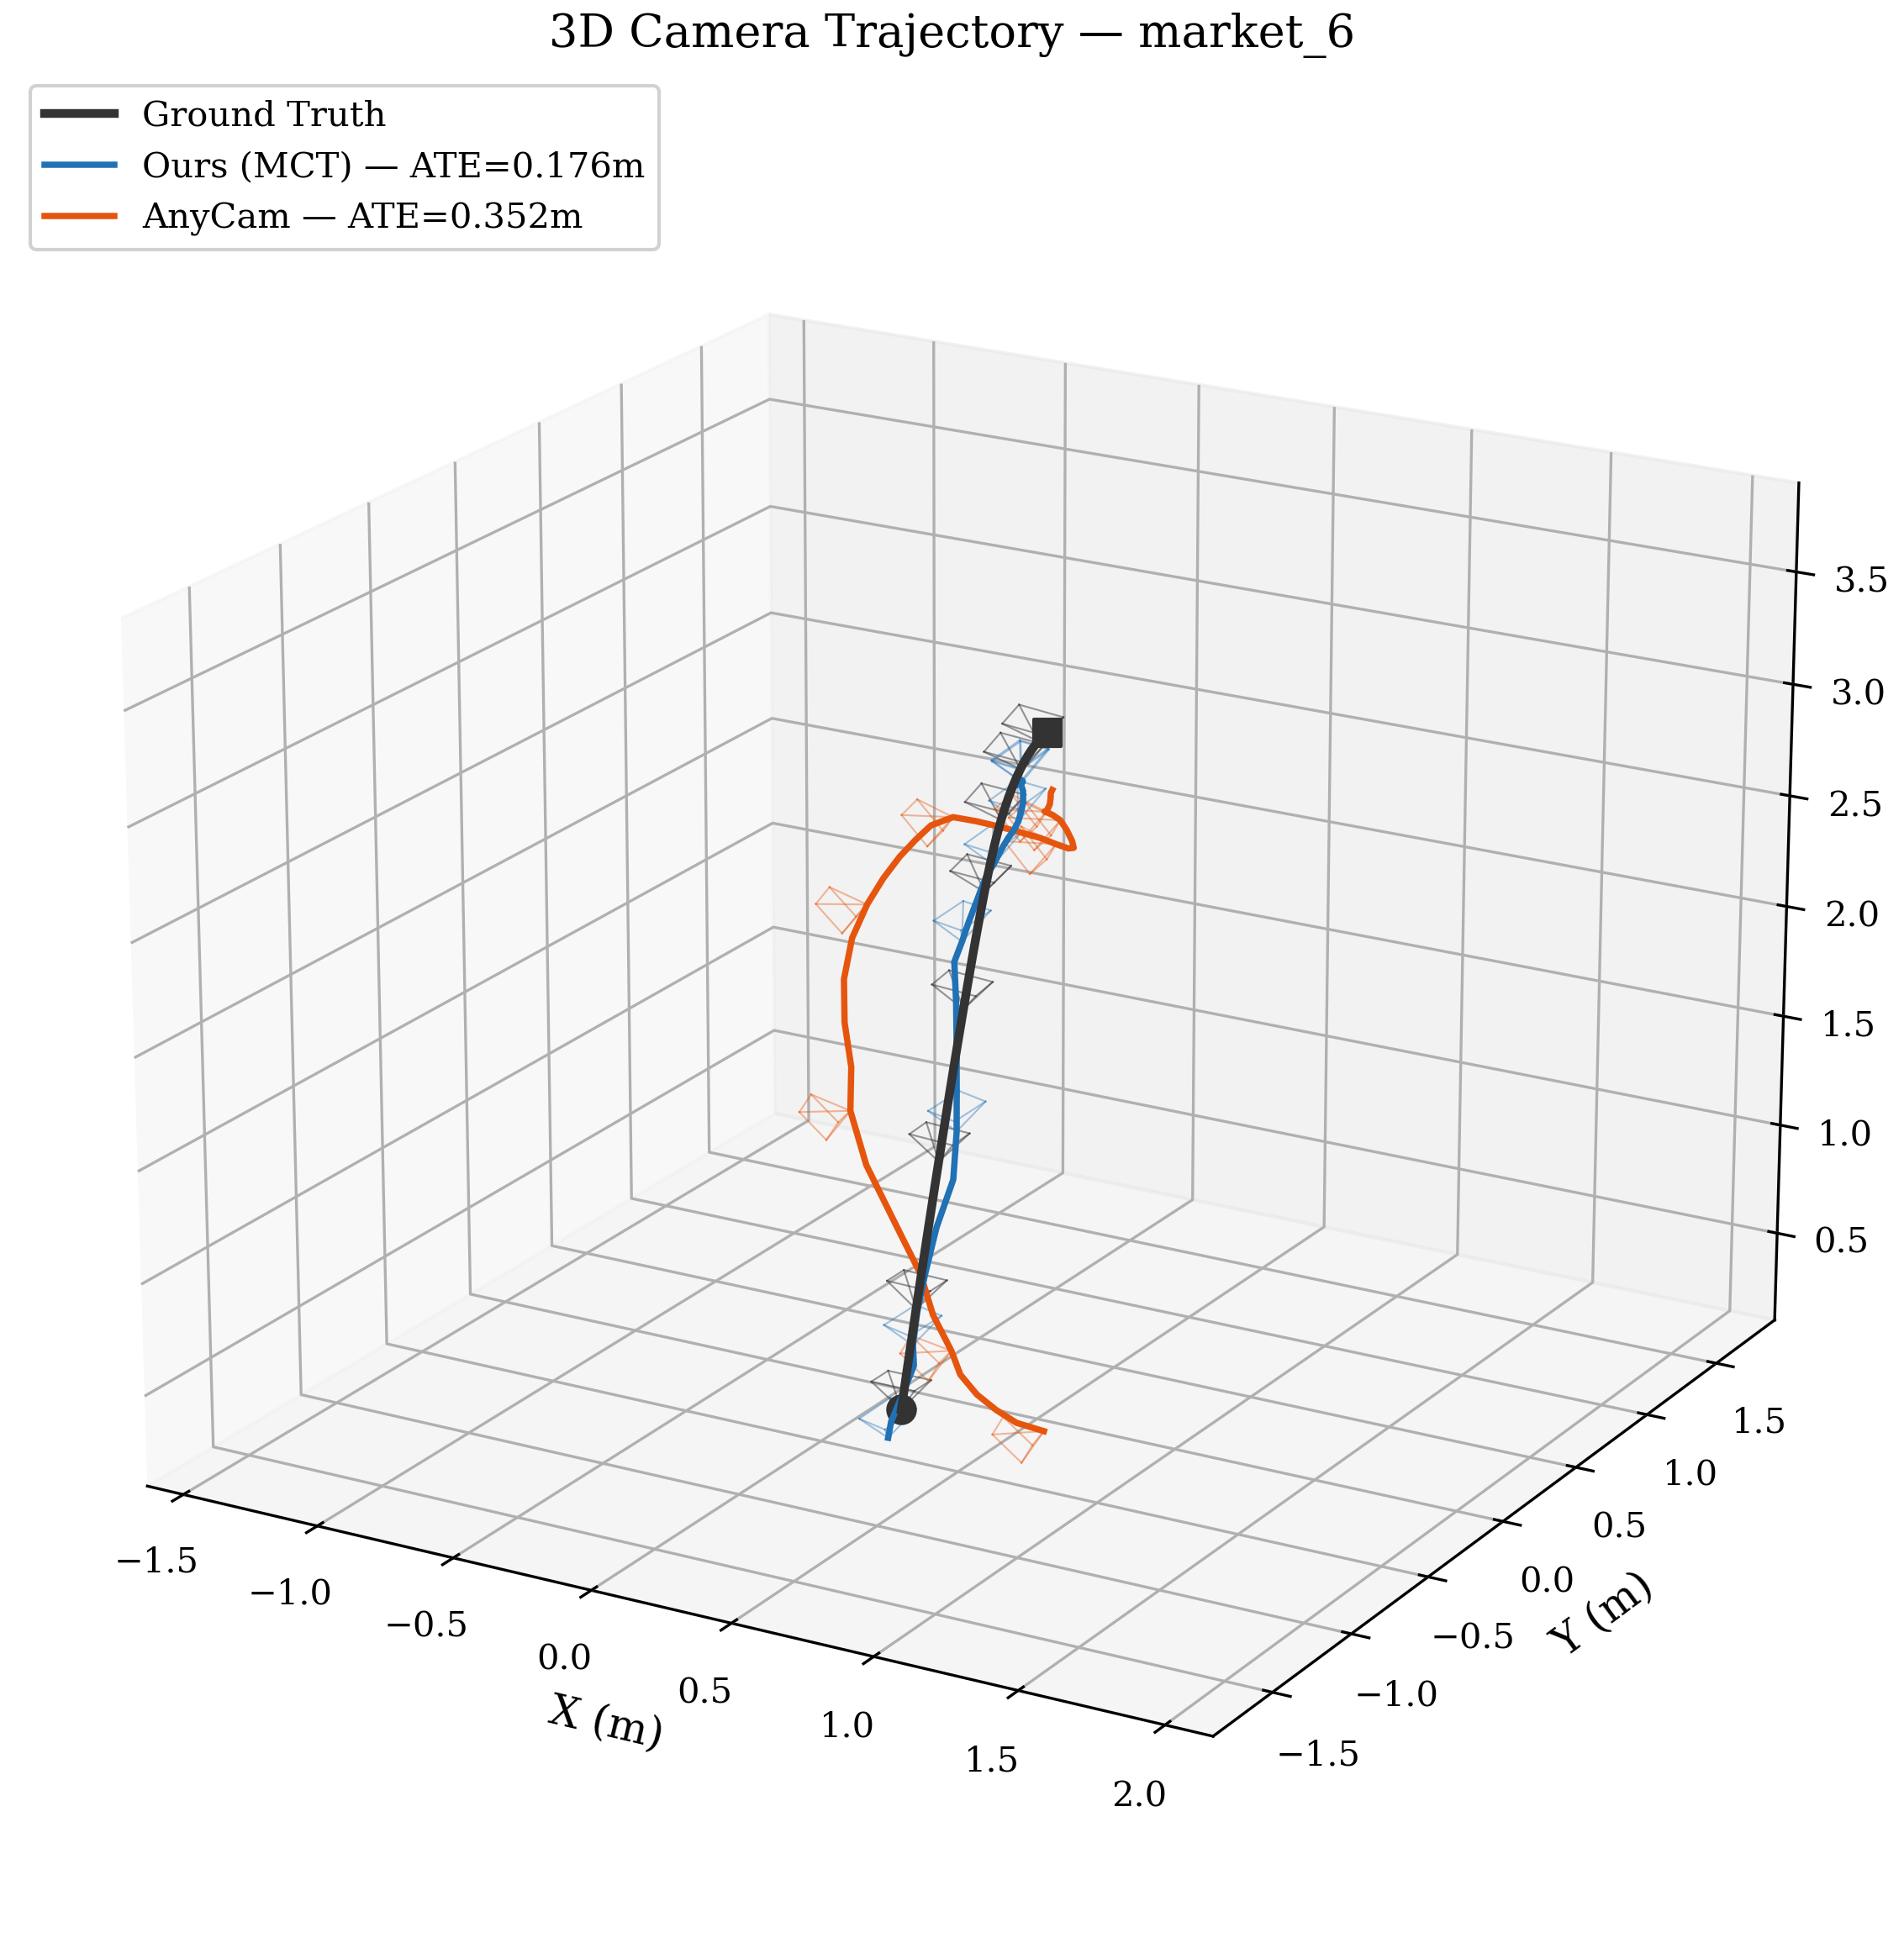
\includegraphics[width=\textwidth,height=0.65\textheight,keepaspectratio]{figures/trajectory_3d_side.png}
\vskip2pt
{\small Sintel \texttt{market\_6}, Sim(3)-aligned.}
\end{column}

\begin{column}{0.43\textwidth}
\textbf{Quantitative:}
\begin{itemize}
  \item Ours ATE: \textbf{0.176\,m}
  \item AnyCam ATE: 0.352\,m
  \item \alert{$2.0\times$ improvement}
\end{itemize}

\vskip6pt
\textbf{Observations:}
\begin{itemize}
  \item Ours (blue) closely follows GT (black)
  \item AnyCam (orange) drifts
\end{itemize}

\vskip4pt
{\small Ours beats AnyCam on 57\% of Sintel sequences.}
\end{column}
\end{columns}

\end{frame}


% ============================================================================
% SLIDE 12: Conclusion & Future Work
% ============================================================================
\begin{frame}{Conclusion \& Future Work}

\textbf{Summary:}
\begin{itemize}
  \item Integrated AnyCalib into AnyCam for accurate, model-agnostic calibration
  \item Multi-Frame Calibration Transformer (MCT) for calibration consistency
  \item Self-supervised, only 7.5\% of parameters trained
  \item \textbf{Up to 31.7\% better rotation, 32.5\% better calibration}
\end{itemize}

\vskip6pt
\textbf{Future work:}
\begin{itemize}
  \item Longer sequences (hierarchical composition, recurrent architectures)
  \item Non-pinhole camera models (fisheye, equirectangular)
  \item Joint depth refinement with calibration and pose
\end{itemize}

\vskip12pt
\centering
{\Large\color{TUMBlue} Thank you! Questions?}

\end{frame}

\end{document}
